\documentclass[
10pt, % Set the default font size, options include: 8pt, 9pt, 10pt, 11pt, 12pt, 14pt, 17pt, 20pt
%t, % Uncomment to vertically align all slide content to the top of the slide, rather than the default centered
aspectratio=169, % Uncomment to set the aspect ratio to a 16:9 ratio which matches the aspect ratio of 1080p and 4K screens and projectors
]{beamer}

\usepackage[all]{xy}

\usepackage[spanish]{babel}
\usepackage[utf8]{inputenc}

\graphicspath{{Images/}{./}} % Specifies where to look for included images (trailing slash required)

\usepackage{booktabs} % Allows the use of \toprule, \midrule and \bottomrule for better rules in tables

%\usepackage{tikz}
%\usetikzlibrary{positioning}
%\usetikzlibrary{shapes,arrows,arrows,positioning,fit}

\usepackage{tikz}
\usetikzlibrary{mindmap}
\usetikzlibrary{arrows, positioning}
\usetikzlibrary{arrows, shapes, positioning, shadows, trees}

\usepackage{forest}

\usepackage{multirow}

\usepackage{graphicx}
\usepackage{hyperref}

\usepackage{xcolor,listings}
\usepackage{textcomp}
%\usepackage{color}

\usepackage{enumitem}

\usepackage{xcolor}

\usepackage{verbatim}
\usepackage{changepage}

\usepackage{algpseudocode}
\usepackage{gensymb}

\usepackage{venndiagram}

\usepackage{graphicx}
% \usepackage{media9}

% \usepackage{algorithm}
% \usepackage{algorithmic}

\providecommand{\abs}[1]{\lvert#1\rvert}

%----------------------------------------------------------------------------------------
%	SELECT LAYOUT THEME
%----------------------------------------------------------------------------------------
\usetheme{Madrid} 

%----------------------------------------------------------------------------------------
%	SELECT COLOR THEME
%----------------------------------------------------------------------------------------
%\usecolortheme{beaver}
%\usecolortheme{seahorse}
\usecolortheme{spruce} % verde suave
%\usecolortheme{whale}
%\usecolortheme{wolverine}

%----------------------------------------------------------------------------------------
%	SELECT FONT THEME & FONTS
%----------------------------------------------------------------------------------------
\usefonttheme{default} % Typeset using the default sans serif font
%\usefonttheme{serif} % Typeset using the default serif font (make sure a sans font isn't being set as the default font if you use this option!)
%\usefonttheme{structurebold} % Typeset important structure text (titles, headlines, footlines, sidebar, etc) in bold
%\usefonttheme{structureitalicserif} % Typeset important structure text (titles, headlines, footlines, sidebar, etc) in italic serif
%\usefonttheme{structuresmallcapsserif} % Typeset important structure text (titles, headlines, footlines, sidebar, etc) in small caps serif

%------------------------------------------------

%\usepackage{mathptmx} % Use the Times font for serif text
%\usepackage{palatino} % Use the Palatino font for serif text

\usepackage{helvet} % Use the Helvetica font for sans serif text
%\usepackage[default]{opensans} % Use the Open Sans font for sans serif text
%\usepackage[default]{FiraSans} % Use the Fira Sans font for sans serif text
\usepackage[default]{lato} % Use the Lato font for sans serif text

%----------------------------------------------------------------------------------------
%	SELECT INNER THEME
%----------------------------------------------------------------------------------------
\useinnertheme{circles}


\setbeamertemplate{footline} % Uncomment this line to remove the footer line in all slides
%\setbeamertemplate{footline}[page number] % Uncomment this line to replace the footer line in all slides with a simple slide count

\setbeamertemplate{navigation symbols}{} % Uncomment this line to remove the navigation symbols from the bottom of all slides

%----------------------------------------------------------------------------------------
%	PRESENTATION INFORMATION
%----------------------------------------------------------------------------------------

\title[Short Title]{Acercamiento al Procesamiento de Sonidos} 

\subtitle{Sistemas de Recuperación de Información}

\author{Lic. Carlos León González \\ Dra.C. Lucina García Hernández}

\institute[UC]{Facultad de Matem\'atica y Computaci\'on \\ Universidad de La Habana \\ \smallskip }

\date{19 de febrero de  2024} % Presentation date or conference/meeting name, the optional parameter can contain a shortened version to appear on the bottom of every slide, while the required parameter value is output to the title slide

%----------------------------------------------------------------------------------------

\begin{document}
	
	\lstset{
		literate=%
		{á}{{\'a}}1
		{í}{{\'i}}1
		{é}{{\'e}}1
		{ý}{{\'y}}1
		{ú}{{\'u}}1
		{ó}{{\'o}}1
		{ě}{{\v{e}}}1
		{š}{{\v{s}}}1
		{č}{{\v{c}}}1
		{ř}{{\v{r}}}1
		{ž}{{\v{z}}}1
		{ď}{{\v{d}}}1
		{ť}{{\v{t}}}1
		{ň}{{\v{n}}}1                
		{ů}{{\r{u}}}1
		{Á}{{\'A}}1
		{Í}{{\'I}}1
		{É}{{\'E}}1
		{Ý}{{\'Y}}1
		{Ú}{{\'U}}1
		{Ó}{{\'O}}1
		{Ě}{{\v{E}}}1
		{Š}{{\v{S}}}1
		{Č}{{\v{C}}}1
		{Ř}{{\v{R}}}1
		{Ž}{{\v{Z}}}1
		{Ď}{{\v{D}}}1
		{Ť}{{\v{T}}}1
		{Ň}{{\v{N}}}1                
		{Ů}{{\r{U}}}1    
	}
	
	
	\begin{frame}
		\titlepage
	\end{frame}
	
	%------------------------------------------------
	% Objetivos
	\begin{frame}
		
		\frametitle{Objetivos}
		
		\begin{itemize}
			\item Identificar los componentes computaciones de las señales de sonidos
			
			\item Comprender los fundamentos del procesamiento de señales de audio a partir del contenido
			
			\item Introducción a los principales extractores de características bajo el dominio del tiempo y la frecuencia
			
		\end{itemize}
		
	\end{frame}
	
	%------------------------------------------------
	% ¿Qué es una señal?
	\begin{frame}
		
		\frametitle{¿Qué es una señal?}
		
		\begin{alertblock}{}
			Una señal, en el contexto del procesamiento computacional de señales, es una representación matemática de un fenómeno físico que varía con respecto al tiempo, al espacio u otra variable independiente. 
		\end{alertblock}
		
	\end{frame}
	
	%------------------------------------------------
	% Representación del sonido
	\begin{frame}
		
		\frametitle{Representación del sonido}
		
		\centering
		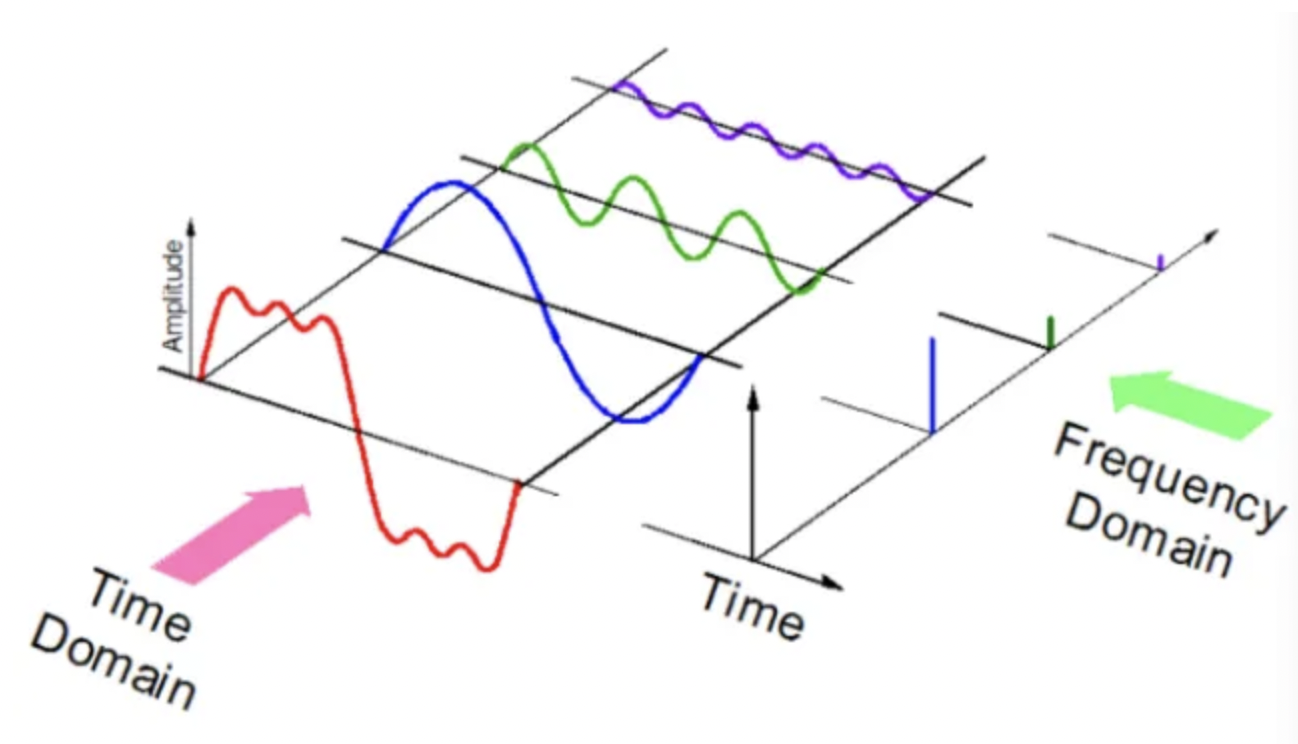
\includegraphics[scale=0.5]{representacion.png}
		
		% Hacer incampié en q son distintos instrumentos
		
	\end{frame}
	
	%------------------------------------------------
	% Espectro
	\begin{frame}
		
		\frametitle{Espectro de la frecuencia del sonido}
		
		
		\begin{alertblock}{}
			Gráfico de intensidad frente a la frecuencia de una onda particular.
		\end{alertblock}
		
		\vspace{1\baselineskip}
		\centering
		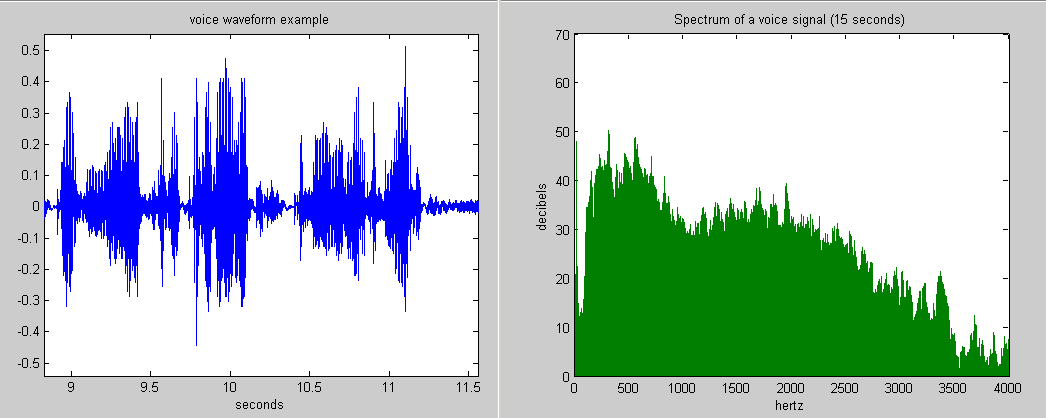
\includegraphics[scale=0.37]{spectrum.png}
		
		{\scriptsize Tomado de \url{https://es.wikipedia.org/wiki/Espectro_de_frecuencias}}
		
		
	\end{frame}
	
	%------------------------------------------------
	% Factores computacionales del sonido
	\begin{frame}
		
		\frametitle{Factores computacionales del sonido}
		
		\begin{itemize}
			
			\item Contenido del sonido
			\begin{itemize} 
				\item Se refiere a todo lo que contiene o no la señal de audio.
				\item Ejemplo: ritmo, timbre, melodía, armonía. 
				% decir de que van cada uno
			\end{itemize}
			
			\item Contexto del sonido
			\begin{itemize} 
				\item Se refiere a la información que no puede inferirse directamente de la señal.
				\item Ejemplo: país de origen, notas del sonido, álbum perteneciente.
			\end{itemize}
			
			\item Propiedades del usuario
			\begin{itemize}
				\item Se refiere a los rasgos de personalidad del oyente.
				\item Ejemplo: preferencias, gustos, conocimiento y  experiencia musicales.
			\end{itemize}
			
			\item Contexto del usuario
			\begin{itemize}
				\item Se refiere al estado actual del usuario.
				\item Ejemplo: ubicación, hora, actividad, estado de ánimo. 
			\end{itemize}
			
		\end{itemize}
		
	\end{frame}
	
	%------------------------------------------------
	% Flujo de trabajo
	\begin{frame}
		
		\frametitle{Etapas para la extracción de información del contenido sonoro}
		
		Pasos para el trabajo de procesamiento computacional con sonidos:
		\begin{enumerate}
			\item Obtención de la señal digital
			\begin{enumerate}[label=1.\arabic*.]
				\item Conversor A/D
				\item Representación matemático-computacional
			\end{enumerate}
			\item Eliminación de ruidos
			\item Extracción de características
		\end{enumerate}
		
	\end{frame}
	
	%------------------------------------------------
	% Conversor A/D
	\begin{frame}
		
		\frametitle{Paso 1: Obtención de la señal digital}
		
		\centering
		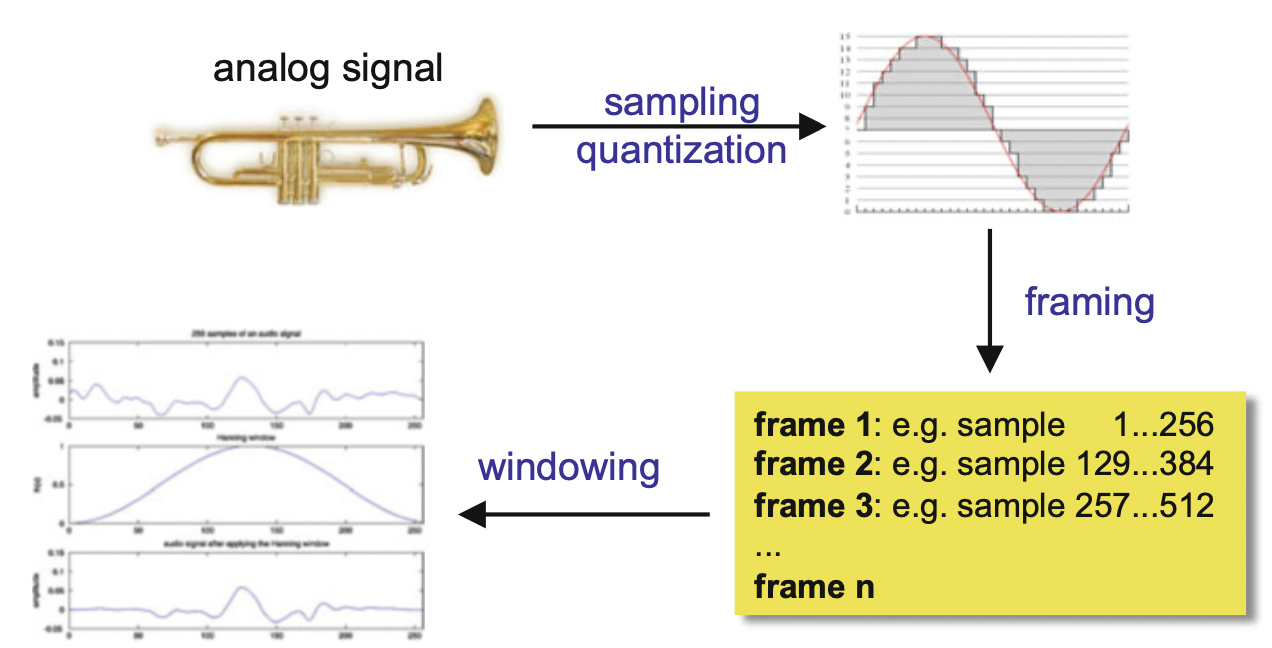
\includegraphics[scale=0.6]{paso1.png}
		
	\end{frame}
	
	%------------------------------------------------
	% Conversor A/D
	\begin{frame}
		
		\frametitle{Conversor A/D}
		
		\begin{alertblock}{}
			Dispositivo o procedimiento para convertir una señal analógica en una señal digital.
		\end{alertblock}
		
		\begin{minipage}{.5\textwidth}
			
			Sobre el dominio del tiempo se establecen intervalos, conocidos como muestras, de modo que se cuantifican los valores tomando un valor representativo del eje y para todo el intervalo. 
			
			\vspace{1\baselineskip}
			Nótese que se produce un error durante el proceso de cuantificación, el cual puede verse como la diferencia entre la curva roja y la curva negra con respecto al eje y.
			
		\end{minipage}%
		\begin{minipage}{.6\textwidth}
			
			\centering
			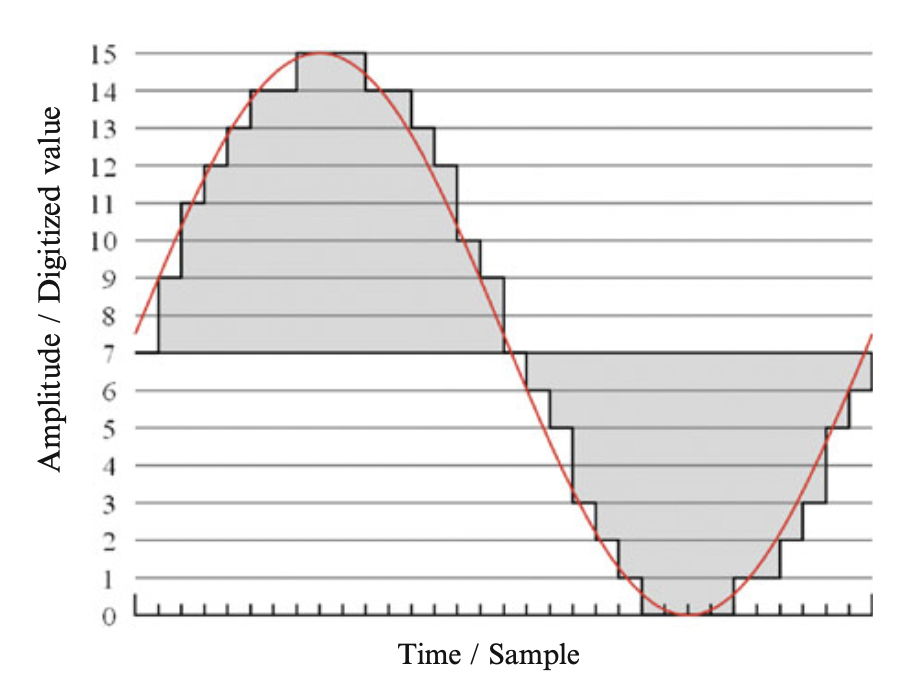
\includegraphics[scale=0.4]{ad.png}
			
			La curva roja representa la señal \\analógica (continua) y la curva negra, la \\señal discreta.
			
		\end{minipage}%
		
		% Muestreo, (sampling)
		% 
		% 	Consiste en tomar diferentes muestras del valor de la señal (tensión, presión,...), la frecuencia con que se realiza el muestreo, se denomina razón o tasa, cuanto mayor sea la frecuencia de muestreo, más fidelidad tendrá la señal digital obtenida.
		% 	
		% 	En el proceso de muestreo se asignan valores numéricos que equivalen al valor de la señal en distintos instantes de tiempo, para así poder realizar a posteriori el proceso de cuantización.
		
		% Cuantización, (quantization)
		% 
		% 	Los valores continuos de la señal se convierten en valores discretos que corresponden a los diferentes niveles de valor (voltaje) que contiene la señal analógica original, lo que permite medirlos y asignarles sus correspondientes valores en el sistema numérico decimal, antes de ser convertidos al sistema binario.
		% 
		% Codificación
		% 
		% 	Los valores así obtenidos de la señal, son representados por códigos previamente establecidos, por lo general la señal digital es codificada en cualquiera de los distintos códigos binarios.
		
	\end{frame}
	
	%------------------------------------------------
	% Ejemplo 
	\begin{frame}
		
		\frametitle{Ejemplo de la obtención de la señal digital (Paso \#1)}
		
		\textcolor{blue}{Ver multimedia \#1}	
		
		\only<2>{
			\vspace{2\baselineskip}
			\textcolor{purple}{¿Cómo reducir el error en el proceso de la descretización de la señal?}
		}
		
	\end{frame}
	
	%------------------------------------------------
	% Marcos y ventanas de la señal
	\begin{frame}
		
		\frametitle{Representación matemático-computacional}
		
		Un marco consiste en un conjunto de muestras consecutivas tomadas en un intervalo de tiempo.\\[4mm]
		
		La selección del tamaño de cada marco no debe de ser menor a los $10 ms$, puesto que ese valor es la menor resolución del oído humano. \\[4mm]
		
		El error producido en el dominio de la frecuencia obstaculiza un eficaz trabajo en el procesamiento de la información que contiene implícitamente la señal. Luego, se necesita una nueva representación que suavice el error, o sea, disminuya la pérdida de información. \\[4mm]

		La aplicación de la Transformada Discreta de Fourier exige una representación periódica de la señal. \\[4mm]
		
		%La TDF necesita un cambio en la representación.
		
		
	\end{frame}
	
	%------------------------------------------------
	% Minimizando el error
	\begin{frame}
		
		\frametitle{Minimizando el error}
				
		La función más utilizada para obtener una señal periódica es la función de Hann, la cual se define como la función de pesos: 
		$$w(k) = 0.5 \cdot (\cos(\frac{2 \cdot \pi \cdot k}{K - 1}))$$
		
		donde \\
		\hspace{.5cm} $K$ es la cantidad de muestras en el marco \\
		\hspace{.5cm} $k \in 1, 2, \cdots, K$
		
	\end{frame}
	
	%------------------------------------------------
	% Aplicación de la función de Hann
	\begin{frame}
		
		\frametitle{Aplicación de la función de Hann a un marco }
		
		\begin{centering}
			
			\only<1>{
				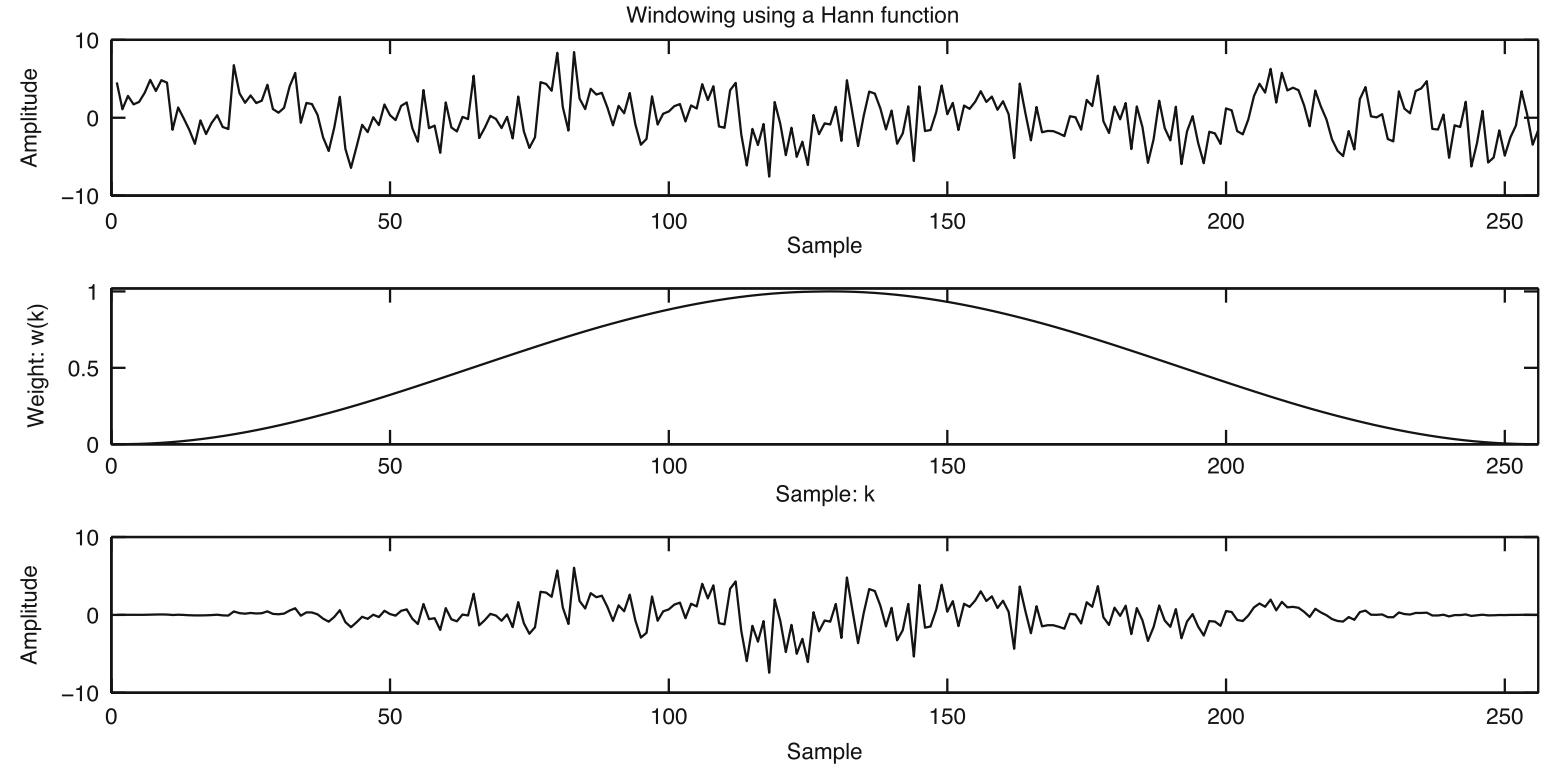
\includegraphics[scale=0.5]{funcion-hann.png}
			}
			
			\only<2>{
				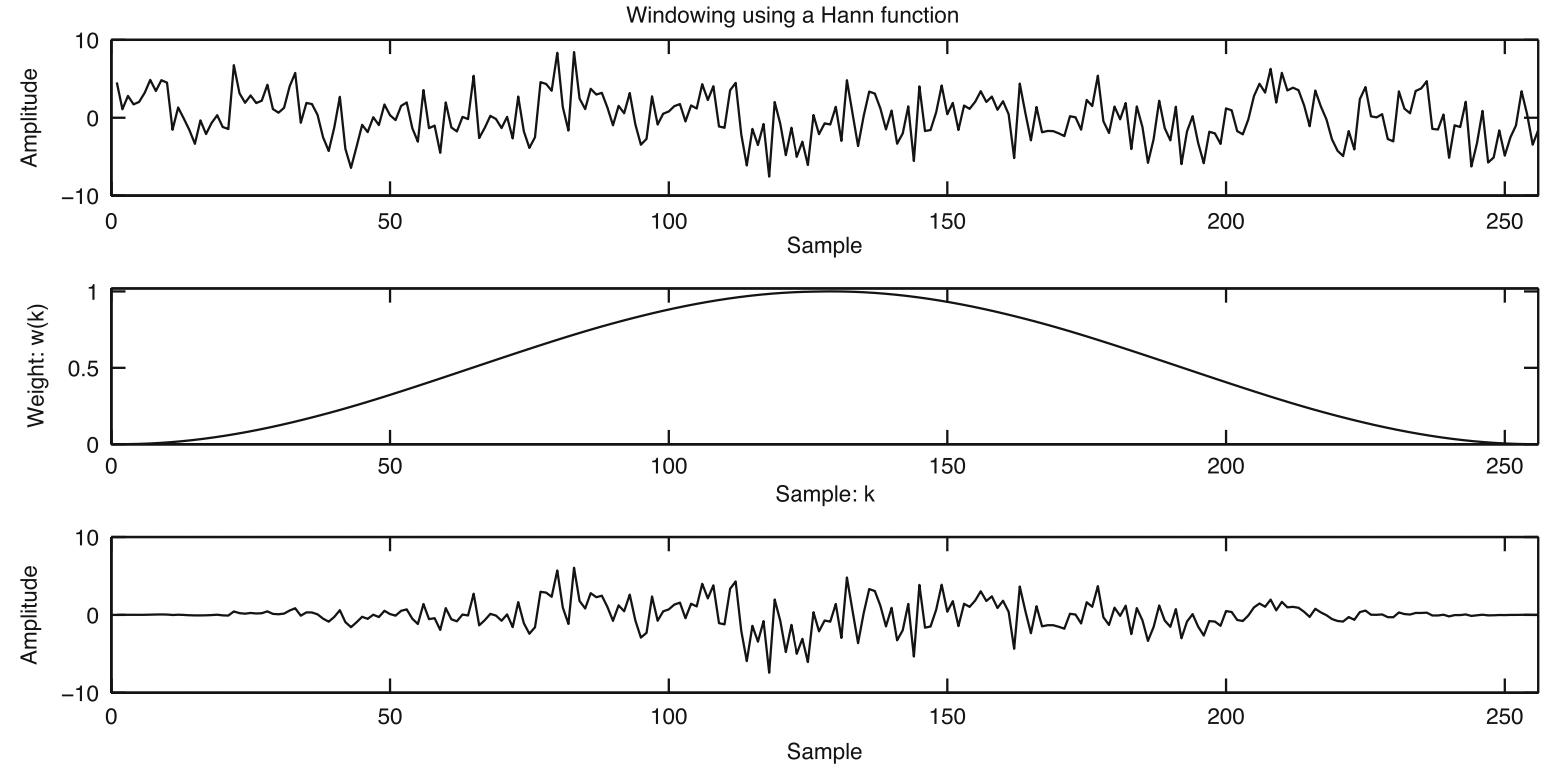
\includegraphics[scale=0.4]{funcion-hann.png}
			}
		
		\end{centering}
		
		\only<2>{
			\vspace{1\baselineskip}
			
			Una ventana es el resultado de aplicar una función a una muestra. \\[2mm]
			
			Para evitar la pérdida de información en los extremos de cada ventana se hace solapar los marcos.
		}
		
	\end{frame}
		
	%------------------------------------------------
	% Paso 2: Eliminación de ruidos
	\begin{frame}
		
		\frametitle{Paso 2: Eliminación de ruidos}
		
		
		\only<1-3>{
			\textcolor{purple}{¿Qué se considera ruido en el tratamiento de los datos que son sonidos?}
		}
		
		\only<2>{
			\vspace{3\baselineskip}
			\textcolor{blue}{Oír multimedia \#3}
		}
		
		\only<3>{
			R:/ En el contexto del sonido, el ruido se refiere a cualquier perturbación o señal no deseada que se superpone a la señal de interés.			
		}
		
		\only<4>{
			\centering
			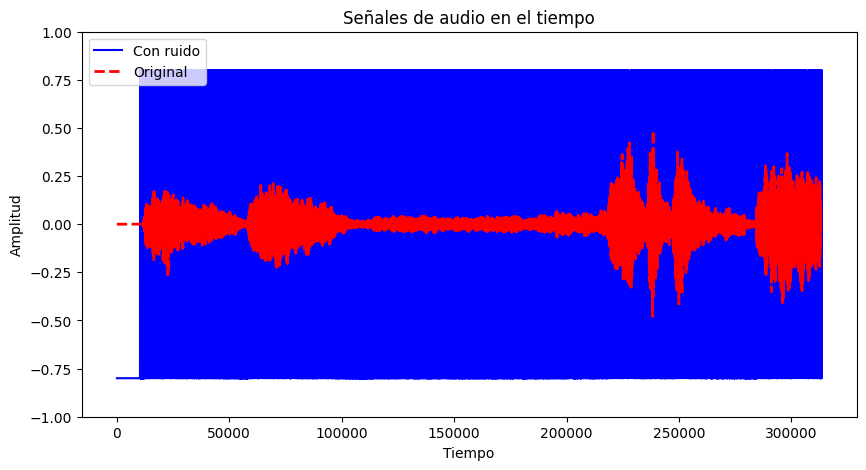
\includegraphics[scale=0.6]{pequenna.png}
			
			\textcolor{blue}{Ver multimedia \#4}
		}
		
	\end{frame}
	
	%------------------------------------------------
	% Mecanismos para eliminar el ruido
	\begin{frame}
		
		\frametitle{Mecanismos para eliminar el ruido}
		
		\begin{itemize}
			
			\item Filtro de paso bajo \\
			Admite señales con frecuencias inferiores a una determinada frecuencia de corte y atenúa señales con frecuencias superiores. 
			
			\pause
			\item Filtro de paso alto \\
			Admite señales con una frecuencias superiores a una determinada frecuencia de corte y atenúa señales con frecuencias inferiores. \\[3mm]
			
			Uno de los filtros más utilizados es la media móvil simple. \\[3mm]
			
			\pause
			\item Filtro adaptativo \\
			Ajusta los parámetros de forma dinámica para adaptarse a las características cambiantes del ruido. El algoritmo LMS (Least Mean Squares, Mínimos Cuadrados Medios) es comúnmente utilizado en filtros adaptativos para reducir el ruido de manera efectiva.
			
			\pause
			\item Otros:
			\begin{itemize}
				\item Substracción espectral
				\item Filtrado de ondaletas
			\end{itemize}
		\end{itemize}
					
	\end{frame}
	%------------------------------------------------
	% Fujo de trabajo
	\begin{frame}
		
		\frametitle{¿Qué se tiene hasta el momento?}
		
		\centering
				
		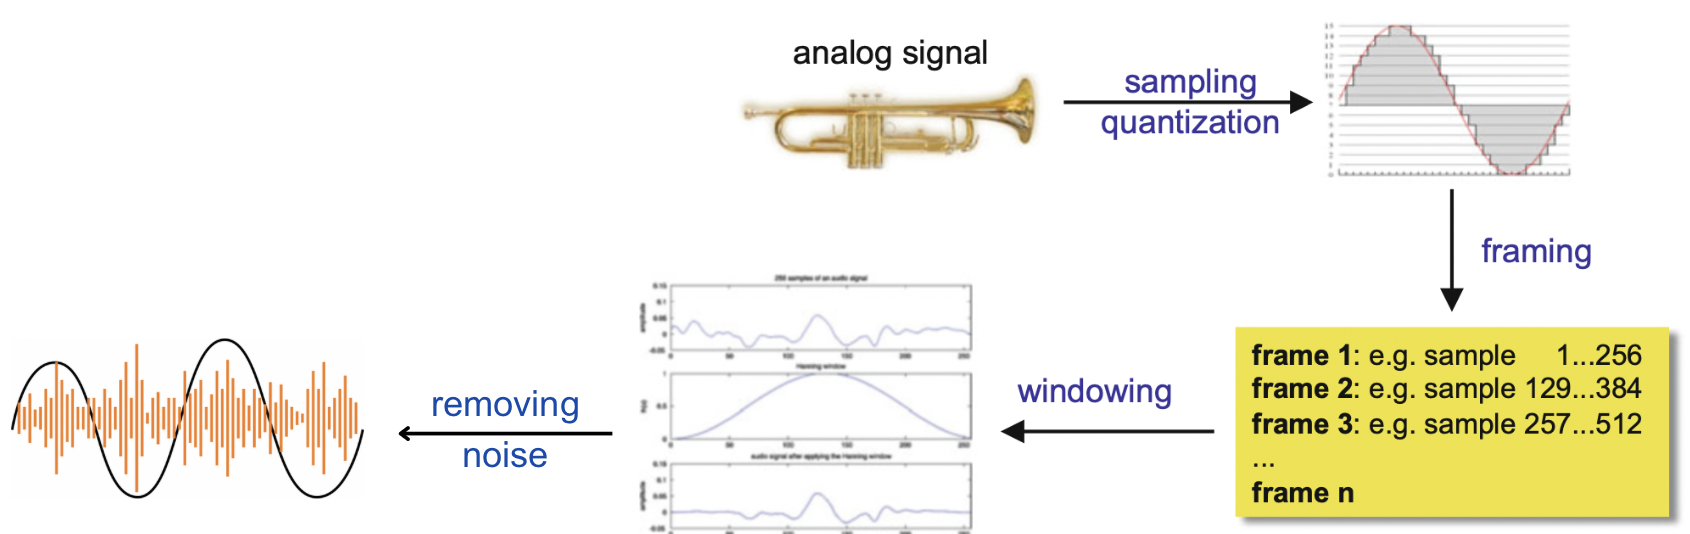
\includegraphics[scale=0.47]{paso1-.png}
		
		\vspace{2\baselineskip}
		
		\pause
		\textcolor{purple}{¿Qué faltaría entonces?}
	
	\end{frame}
	
	%------------------------------------------------
	\begin{frame}
		
		\frametitle{Paso 3: Extracción de características}
		
		\centering
		
		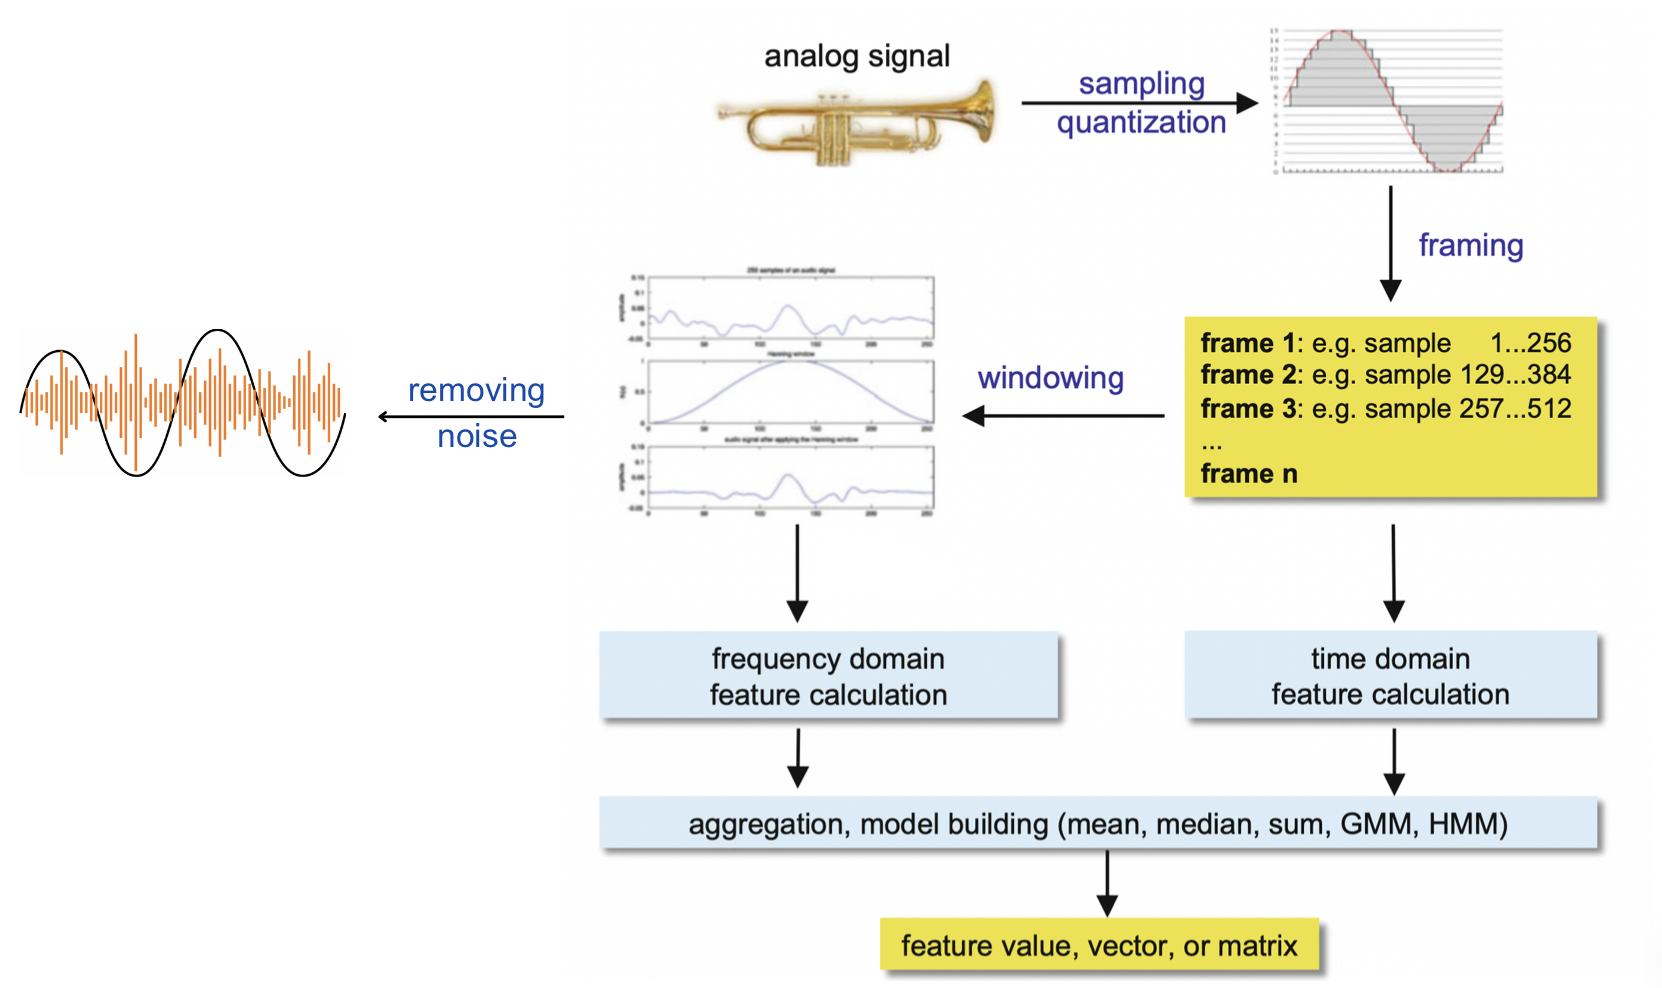
\includegraphics[scale=0.44]{todo.png}
		
		% desplegar qué es GMM (modelos mixtos gausianos) y hmm (modelos de markov oculto)
		
	\end{frame}
	
	%------------------------------------------------
	% Paso 3: Extracción de características 
	\begin{frame}
		
		\frametitle{Paso 3: Extracción de características}
		
		Niveles de abstracción de las características:
		\begin{itemize}
			\item Bajo nivel 
			\only<2>{
				\begin{itemize}
					
					\item Dominio del tiempo
					\begin{itemize}
						\item Cobertura de la amplitud
						\item Energía cuadrática media 
					\end{itemize}
					
					\item Dominio de la frecuencia 
					\begin{itemize}
						\item Razón de energía de banda
						\item Centroide espectral
					\end{itemize}
					
				\end{itemize}
			}
			
			\item Nivel medio
			
			\item Alto nivel
			
		\end{itemize}
		
	\end{frame}
	
	%------------------------------------------------
	% Amplitud envolvente
	\begin{frame}
		
		\frametitle{Dominio del tiempo. Cobertura de la amplitud}
		
		Amplitud máxima entre todas las muestras de un marco $t$. Se define como:
		
		$${AE}_t = \max_{k=tK}^{(t+1) \cdot K-1} s(k)$$
		
		donde $s(k)$ es la amplitud de la $k$-ésima muestra del marco $K$. \\[2mm]
		
		La representación es muy sensible a valores atípicos.
		
		\vspace{1\baselineskip}
		\centering
		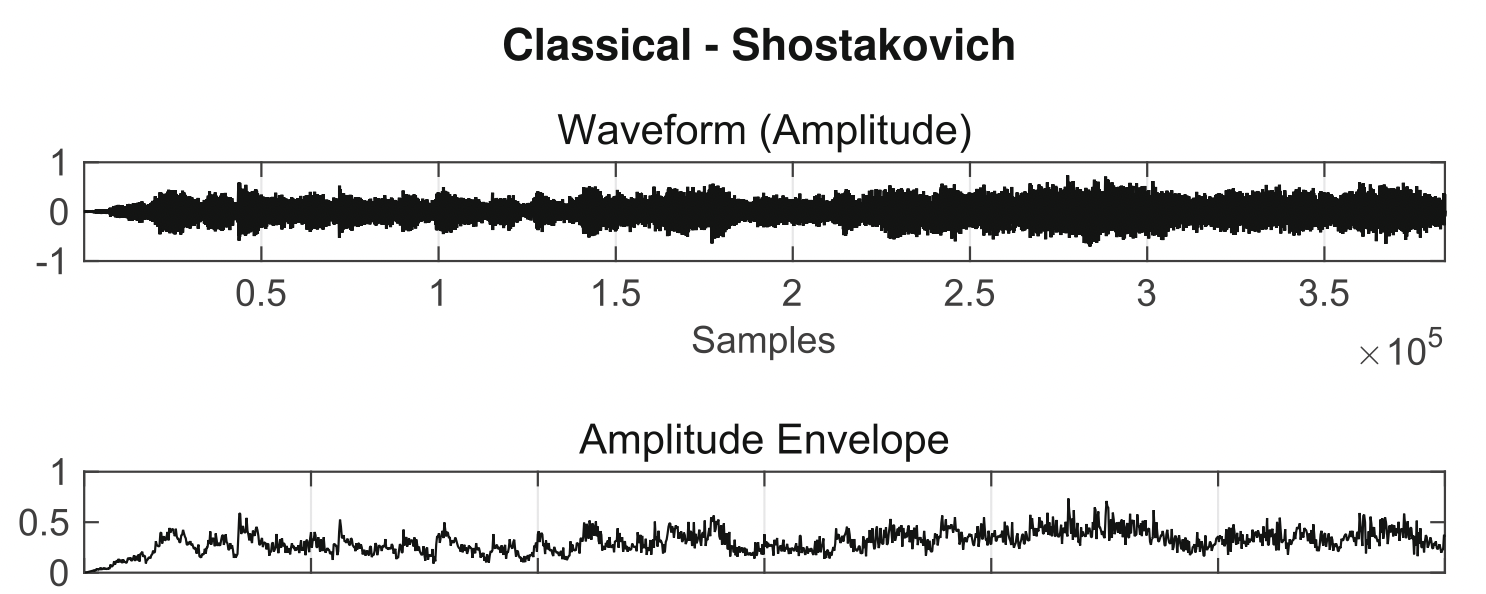
\includegraphics[scale=0.4]{ae.png}
		
	\end{frame}
	
	%------------------------------------------------
	% Energía cuadrática media
	\begin{frame}
		
		\frametitle{Dominio del tiempo. Energía cuadrática media}
		
		% RMS energy, level or power (potencia)
		
		Indicador de nuevos eventos en la segmentación del audio y se relaciona con la intensidad del sonido. Se define como:
		
		$${RMS}_t = \sqrt{\frac{1}{K} \sum_{k=tK}^{(t+1)(K-1)} s(k)}$$
		
		\vspace{1\baselineskip}
		\centering
		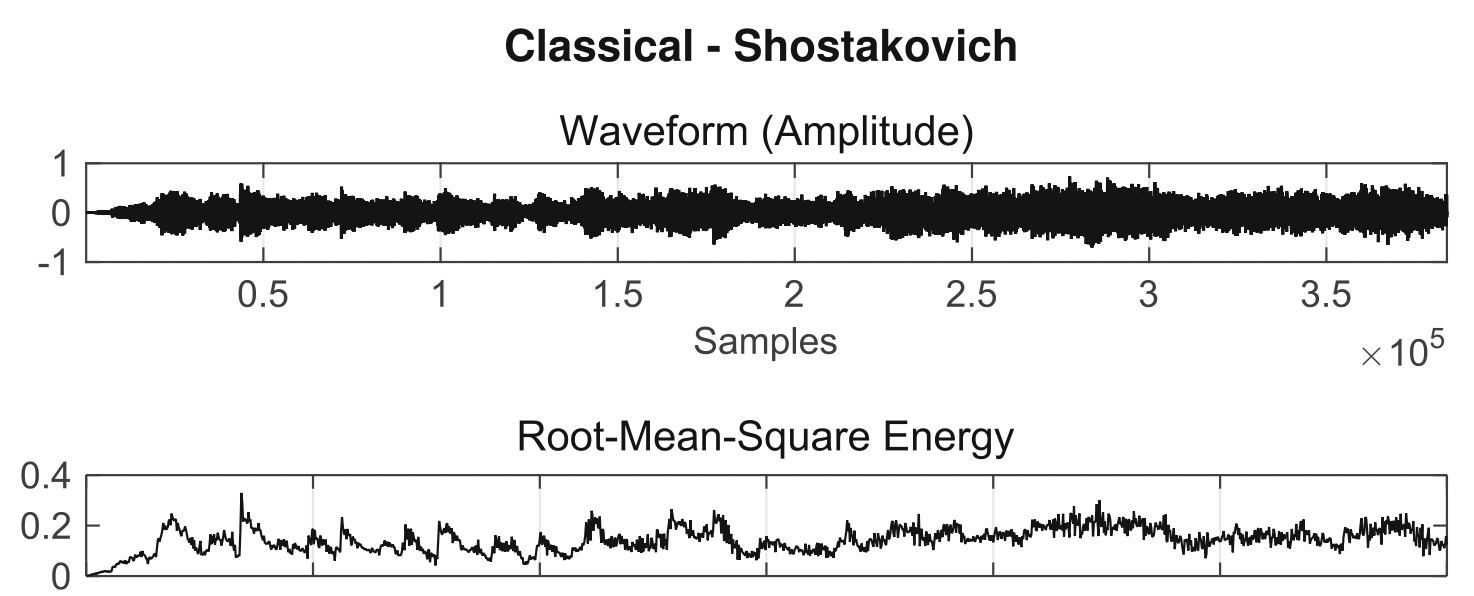
\includegraphics[scale=0.4]{rms.png}
		
	\end{frame}
	
	%------------------------------------------------
	% Relación de energía de banda
	\begin{frame}
		
		\frametitle{Dominio de la frecuencia. Razón de potencia de banda}
		
		\only<1>{
			Una banda de frecuencia es un intervalo en el dominio de la frecuencia delimitado por una frecuencia baja y una alta. \\[4mm]
		
			\begin{centering}
				
				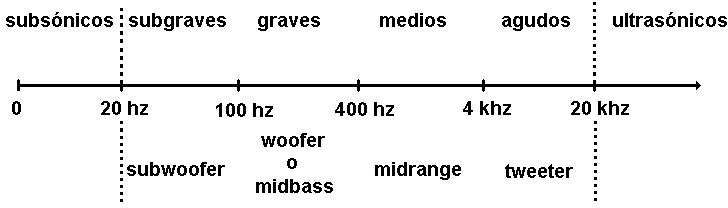
\includegraphics[scale=0.45]{banda.jpg}
				
				{\scriptsize Tomado de \url{http://cienciasfera.com/materiales/tecnologia/tecno02/tema13/2\_tipos\_de\_seales.html}}
				
			\end{centering}
		}
		
		\only<2->{
			La razón de potencia de banda relaciona las bandas de bajas frecuencias con las de altas frecuencias, midiendo cuán dominantes son las bandas de baja frecuencia. Se define como:
			
			$${BER}_t = \frac{\sum_{n=1}^{F-1} m_t(n)^2}{\sum_{n=F}^{N} m_t(n)^2}$$
		}
		
		
		\only<3>{
			donde \\
			\hspace{.5cm} $m_t(n)$ representa la magnitud de la señal en el dominio de la frecuencia en el marco $t$ y en la banda de frecuencia $n$. \\
			\hspace{.5cm} $F$ representa la banda de frecuencia que divide las bandas de menor frecuencia entre las bandas de mayor frecuencia. \\
			\hspace{.5cm} $N$ representa la cantidad total de bandas. \\[3mm]
			
			BER es utilizada en la discriminación de la voz/música para la clasificación del género de la música. 
		}
		
		\only<4->{
			\vspace{1\baselineskip}
			\centering
			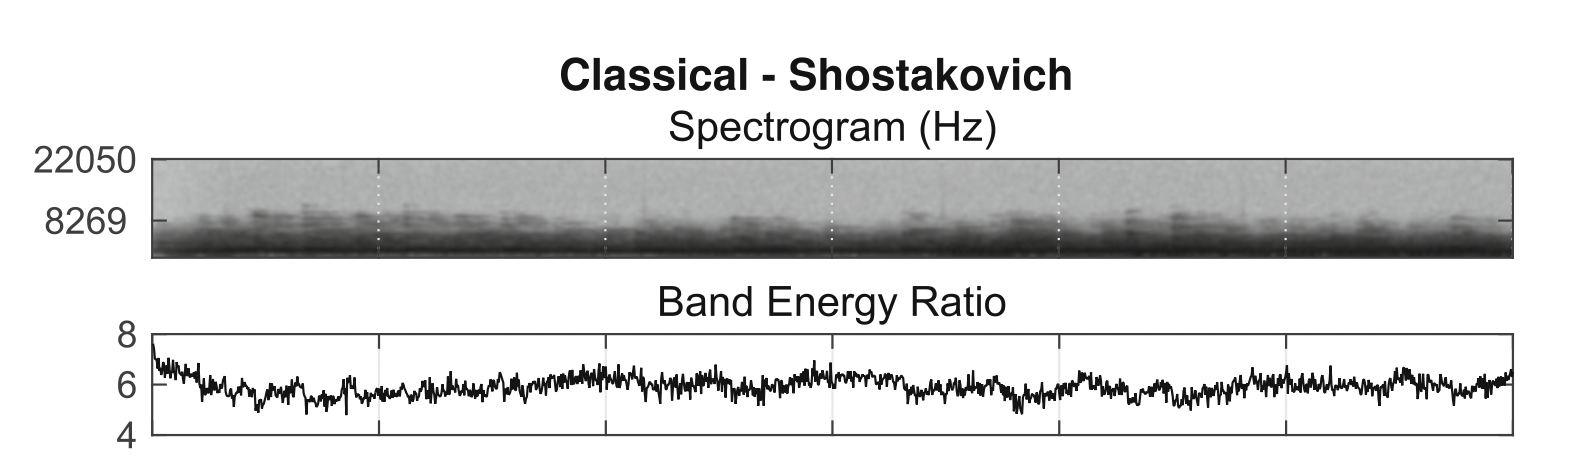
\includegraphics[scale=0.45]{ber.png}
		}
		
	\end{frame}
	
	%------------------------------------------------
	% Centroide espectral 
	\begin{frame}
		
		\frametitle{Dominio de la frecuencia. Centroide espectral}
		
		Representa la banda de frecuencia donde se concentra la mayor parte de la potencia. Se define como:  		
		
		$${SC}_t = \frac{\sum_{n=1}^{N} m_t(n) \cdot n}{\sum_{n=1}^{N} m_t(n)}$$
		
		Se utiliza como medida del ``brillo'' de un sonido, que se relaciona con el timbre musical. Sin embargo, SC es muy sensible al filtrado de paso bajo ya que a las bandas de alta frecuencia se les da más peso que a las bajas. Esto es particularmente problemático cuando la cantidad de muestras es pequeña.
		
		% En las piezas clásicas se muestran valores para SC más bajos y con diferencia los más estables, mientras que el SC fluctúa mucho más que las canciones Electrónicas y Metal. Esto evidencia la “claridad” o “brillo” del sonido en la pieza para piano (monofónica) de Shostakovich, en contraste con las piezas de otros géneros.
		
		\centering
		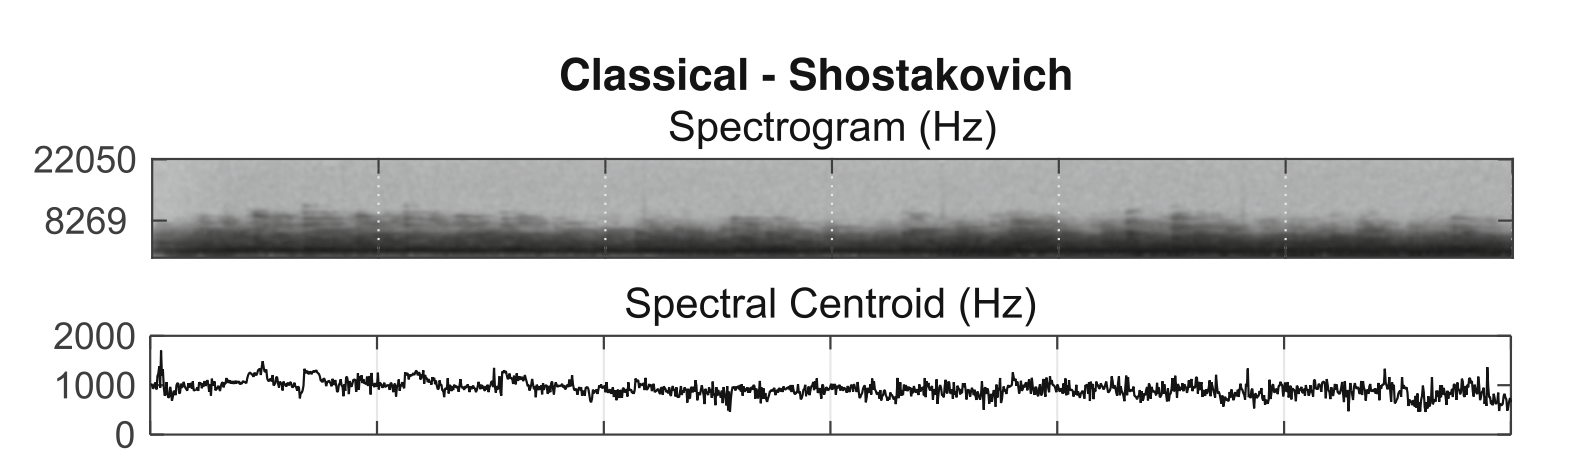
\includegraphics[scale=0.45]{sc.png}
		
	\end{frame}
	
	%------------------------------------------------
	% Paso 3: Extracción de características 
	\begin{frame}
		
		\frametitle{Paso 3: Extracción de características}
		
		Niveles de abstracción de las características:
		\begin{itemize}
			\item \textcolor{gray}{Bajo nivel}
		
			\item Nivel medio
			
				\only<2>{
				\begin{itemize}
					\item Utilizando marcos
					\begin{itemize}
						\item Coeficientes cepstrales de frecuencia Mel
					\end{itemize}
					
					\item Utilizando bloques
					\begin{itemize}
						\item Patrón espectral
					\end{itemize}
					
				\end{itemize}
			}
			
			\item Alto nivel
			
		\end{itemize}
		
	\end{frame}
	
	%------------------------------------------------
	% Coeficientes cepstrales de frecuencia Mel
	\begin{frame}
		
		\frametitle{Coeficientes Cepstrales en las Frecuencias de Mel}
		
		% Tienen su rigen en el procesamiento del habla, pero se ha descubierto que son adecuados para modelar el timbre de la voz.  \\[3mm]
		Permite la modelación del timbre de la voz. \\[5mm]

		Procedimiento para obtener los coeficientes:
		\begin{enumerate}
			\item Aplicar la transformada de Fourier a las frecuencias de un marco de una señal para obtener un espectro representado en Hz.
			
			\item Convertir el espectro hallado a la escala de Mel.
			
			\item Al espectro representado en la escala de Mel se le aplica la función logaritmo y se computa la transformada del coseno discretizada.
			
			\item El resultado es un conjunto de vectores de coeficientes MFCCs.\\[4mm]
		\end{enumerate} 
		
		\pause
		Los vectores MFCCs describen las periodicidades encontradas sobre el dominio de la frecuencia dado un marco. 

		% Mel viene de la melodía, se basa en la percepción humana de los tonos. Es una escala musical perceptual de tonos juzgados como intervalos equiespaciados por parte de observadores.
	
	\end{frame}
	
	%------------------------------------------------
	% Coeficientes cepstrales de frecuencia Mel
	\begin{frame}
		
		\frametitle{Coeficientes Cepstrales en las Frecuencias de Mel (MFCCs)}
						
		Calcular los vectores MFCC u otras características a nivel de marco para una pieza musical completa generalmente produce varias decenas de miles de vectores de características individuales. \\[3mm]
		
		La agregación de esta gran cantidad de vectores de características generalmente se realiza mediante un resumen estadístico de los vectores resultantes, aplicando cuantificación de vectores o ajustando modelos probabilísticos. \\[3mm]
		
		Todos los métodos proporcionan representaciones de la distribución de los vectores MFCC en toda la pieza.  \\[3mm]
			
		\only<2>{
			\textcolor{purple}{¿A qué se parece esto?}
		}
		
		\only<3>{
			\textcolor{orange}{¡Bolsa de palabras!} \\[2mm]
			
			Aunque en procesamiento de sonidos se le llama \textbf{bolsa de marcos}.
		}
		
	\end{frame}
	
	%------------------------------------------------
	% Ejemplo de MFCCs 
	\begin{frame}
		
		\frametitle{Ejemplo de MFCCs}
		
		\centering
		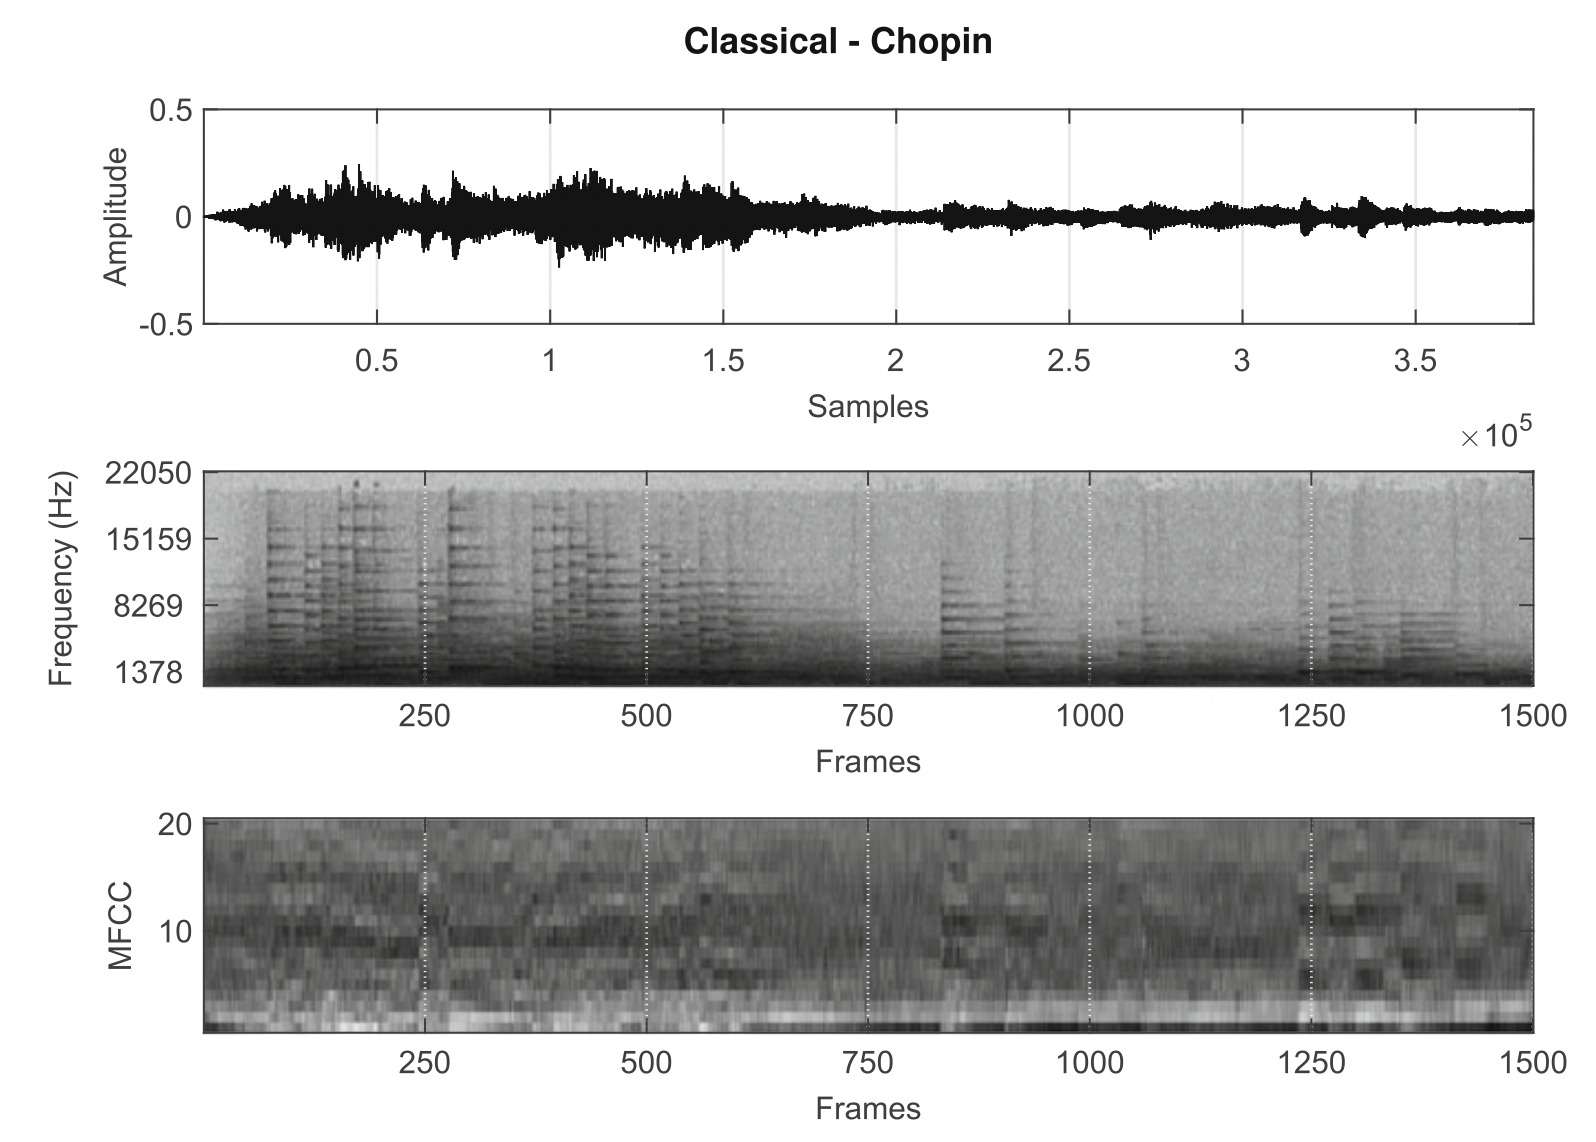
\includegraphics[scale=0.39]{mfcc.png}
		
	\end{frame}
	
	%------------------------------------------------
	% Patrón espectral
	\begin{frame}
		
		\frametitle{Patrón espectral}
		
		\begin{minipage}{.5\textwidth}
			
			Un bloque se define como un conjunto de marcos consecutivos. \\[1.5mm]
			
			El patrón espectral es un método que se aplica sobre los espectogramas, de modo que extrae bloques de longitud fija que se procesan una a la vez. \\[1.5mm]
			
			Las frecuencias se miden en la escala Cent, agrupadas en 98 bandas. \\[1.5mm]
			% Cent es la menor unidad que usualmente se emplea para medir intervalos musicales.
			
			% Las características a nivel de bloques describen segmentos largos de una pieza musical, generalmente segundos. \\[1.5mm]
			
			Esta método se relaciona con el timbre. 
			
		\end{minipage}%
		\begin{minipage}{.58\textwidth}
			
			\centering
			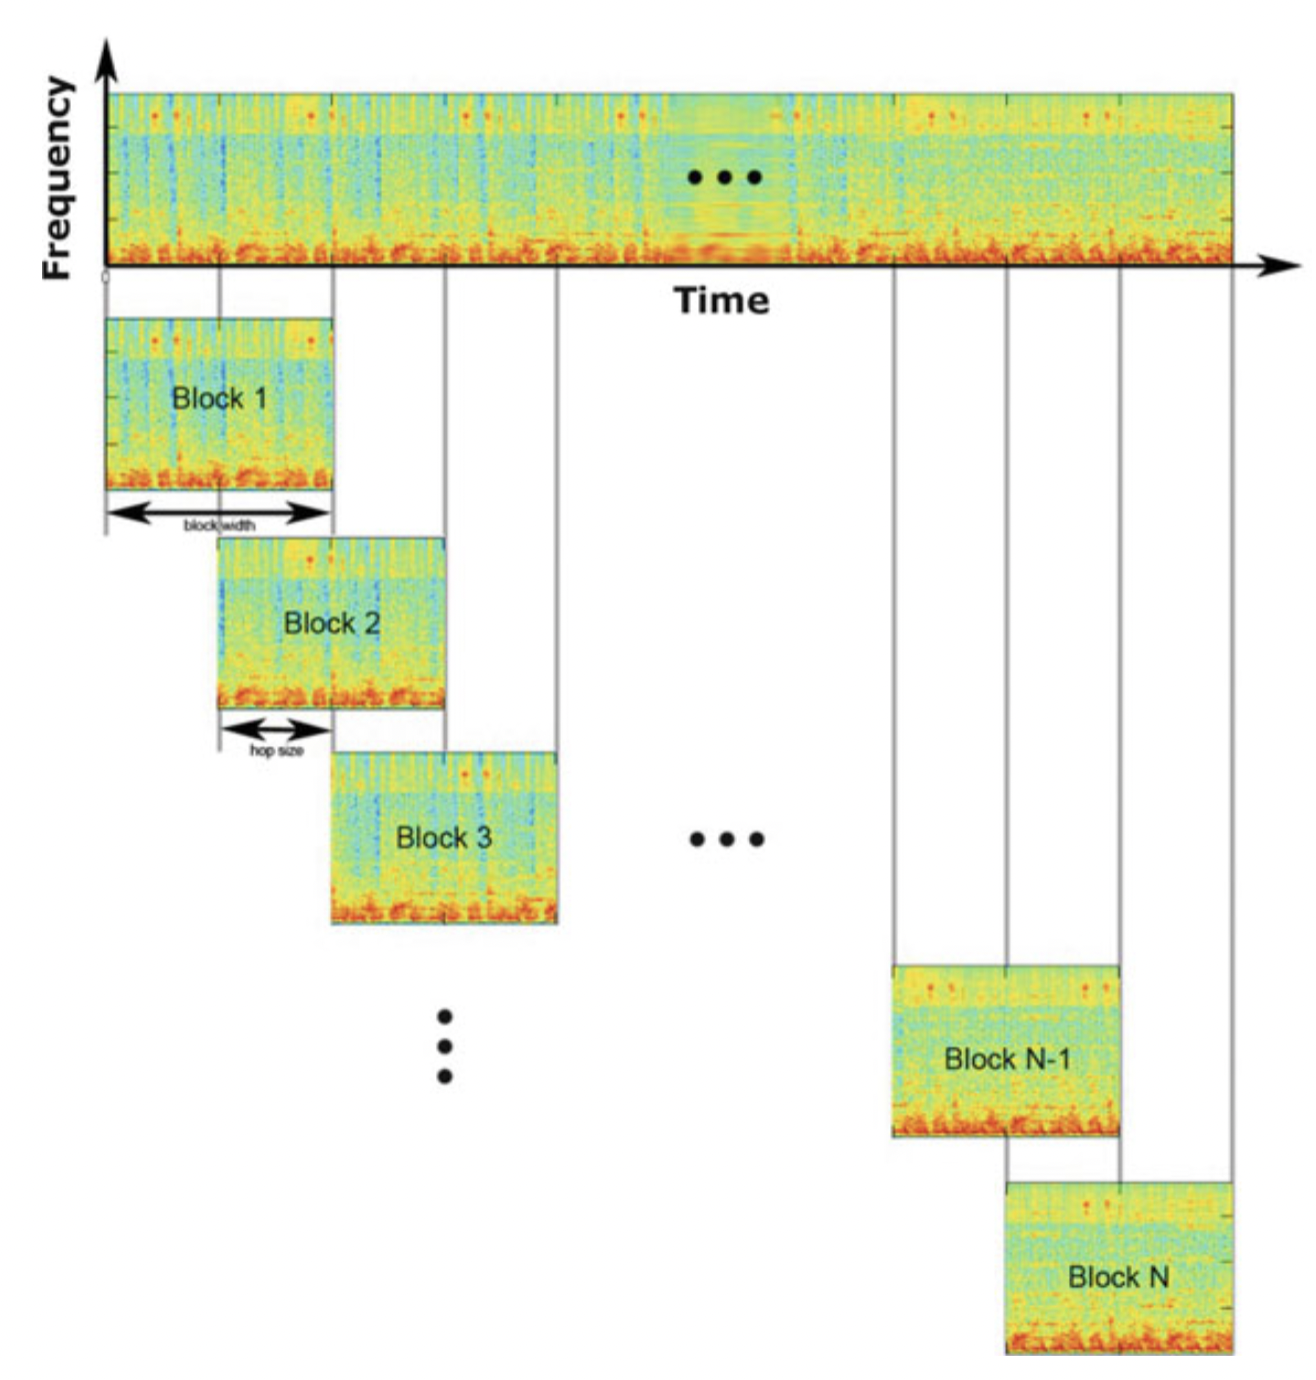
\includegraphics[scale=0.3]{bloque.png}
			
		\end{minipage}%	
		
	\end{frame}
	
	%------------------------------------------------
	% Patrón espectral
	\begin{frame}
		
		\frametitle{Patrón espectral}
		
			El orden definido sobre las bandas de frecuencia en cada marco genera dimensiones. \\[2mm]
			
			El patrón espectral de una pieza musical se calcula como el $90\%$ sobre cada dimensión para todos los bloques. 
						
			\vspace{2\baselineskip}
			
			\centering
			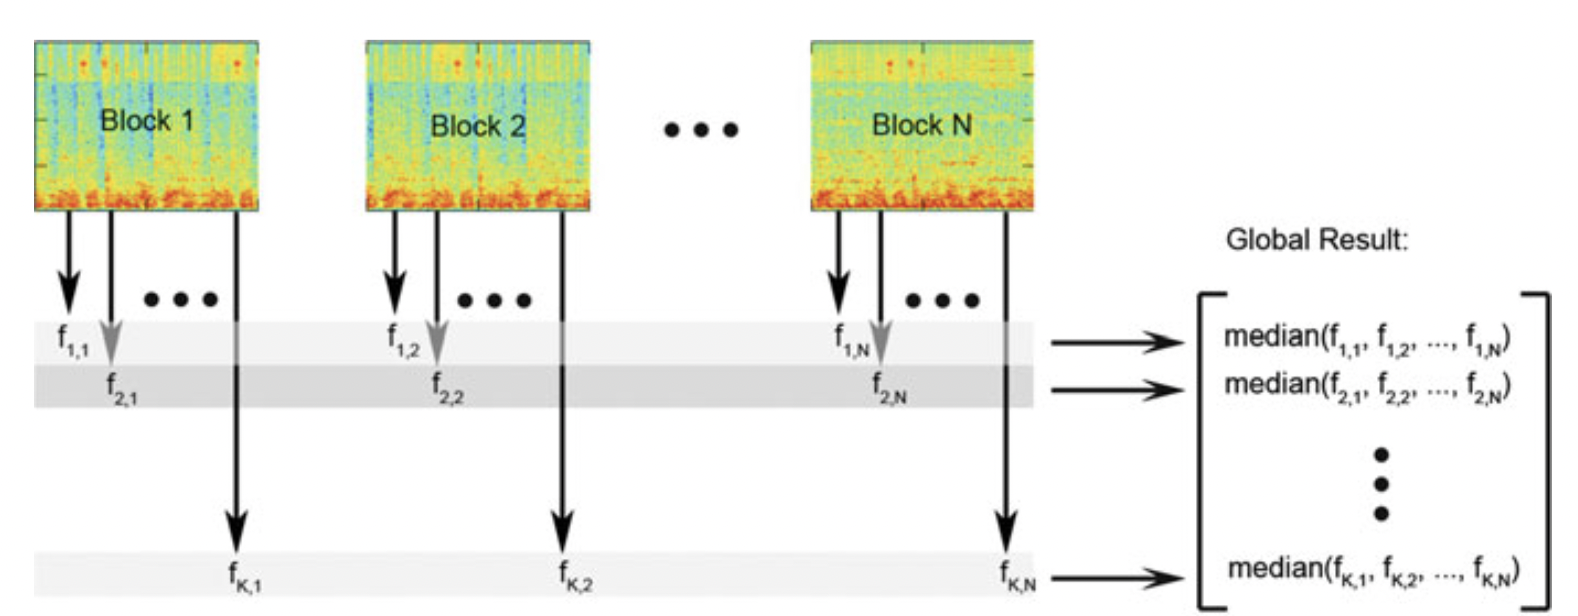
\includegraphics[scale=0.4]{patron-espectral.png}
			
	\end{frame}
	
	%------------------------------------------------
	% Paso 3: Extracción de características 
	\begin{frame}
		
		\frametitle{Paso 3: Extracción de características}
		
		Niveles de abstracción de las características:
		\begin{itemize}
			\item \textcolor{gray}{Bajo nivel}
		
			\item \textcolor{gray}{Nivel medio}
			
			\item Alto nivel
			
			\begin{itemize}
				\item Ritmo
				\item Género
				\item Melodía
				\item Instrumentos
			\end{itemize}
			
		\end{itemize}
		
	\end{frame}
	
	%------------------------------------------------
	% Break
	{
		\setbeamertemplate{background canvas}
		{%
			
\includegraphics[width=\paperwidth,height=\paperheight]{mucho.png}
		}
		
		\begin{frame}
		\end{frame}
	}
	
	%------------------------------------------------
	% Aplicaciones
	\begin{frame}
		
		\frametitle{Aplicaciones del procesamiento del contenido de los  sonidos}
		
		\begin{itemize}
			\item Recuperación relacionada con la música
			\begin{itemize}
				\item Reconocimiento del instrumento
				\item Clasificación del estilo de la música
				\item Similaridad en la música				
			\end{itemize}
			
			
			\item Recuperación relacionada con el habla
			\begin{itemize}
				\item Reconocimiento y transcripción del contenido de programas de radio, conversación telefónica, grabación de reuniones
			\end{itemize}
			
			\item Otras aplicaciones de recuperación de audio
			\begin{itemize}
				\item Alarmas
				\item Sonidos naturales
				\item Impacto del sonido en el sueño
			\end{itemize}
			
		\end{itemize}
		
	\end{frame}
		
	%------------------------------------------------
	% Conclusiones
	\begin{frame}
		
		\frametitle{Conclusiones}
		
		\begin{itemize}
			\item Los sonidos 
			\begin{itemize}
				\item no solo son documentos.
				\item no solo son información acústica.
				\item  son huellas del entorno (personas, animales, dispositivos, etc.).
			\end{itemize}
			
			\vspace{1\baselineskip}
			
			\item Existen una variedad de técnicas y enfoques para abordar la recuperación de información en sonidos, que van desde algoritmos clásicos de procesamiento de señales hasta técnicas modernas de aprendizaje automático y minería de datos. La elección de la técnica adecuada depende del contexto específico y de los requisitos de la aplicación.
			
			\vspace{1\baselineskip}
						
			\item La comprensión del procesamiento computacional de señales de audio para la recuperación de información tiene aplicaciones prácticas y relevantes en una amplia variedad de campos, incluyendo la música, la medicina, la seguridad, la comunicación y el entretenimiento.
			
		\end{itemize}
		
	\end{frame}
	
	%------------------------------------------------
	% Bibliografía
	\begin{frame}
		
		\frametitle{Bibliografía}
		
		\begin{itemize}
			\item Knees, Peter; Schedl, Markus. Music Similarity and Retrieval. An Introduction to Audio- and Web-based Strategies. The Information Retrieval Series 36. 2016.
			
			\item \url{https://medium.com/clasificación-de-música-a-través-del-análisis-de/clasificación-de-música-a-través-del-análisis-de-señales-de-audio-1da23481b47c}
			
		\end{itemize}
		
	\end{frame}
	
	%------------------------------------------------
	% Fin
	\begin{frame}
		\titlepage
	\end{frame}
	
	
	
\end{document} 